\section{Clasificación de funciones}
$f : D \subset R^n \to R^m$

\begin{figure}[H] 
    \centering    
    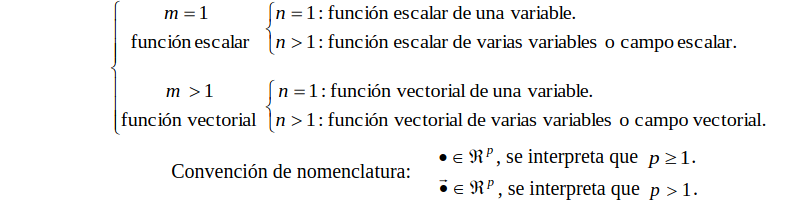
\includegraphics[width=0.8\textwidth]{img/funciones.png}
    \label{fig:funciones}
\end{figure}

\subsection{Funciones vectoriales}
Las funciones vectoriales son de tipo 
$f = (f_1, f_2, \ldots, f_m): D \subset R^n \to R^m$ con $m > 1$. Donde cada componente $f_i$ 
con $i = 1, \ldots, m$ es una función escalar definida en $D$.

$$
f_i : D \subset R^n \to R \quad \text{con } i = 1, \ldots, m
$$

\subsection{Representaciones geométricas de una función escalar}

Sea
$f : D \subset R^n \to R$, se denomina gráfica de $f$ al conjunto
$G_f \subset R^{n+1}$
definido por:

$$
G_f \doteq \{   
    (x_1, \ldots, x_n, u) \in R^{n+1} \mid (x_1, \ldots, x_n) \in D, u = f(x_1, \ldots, x_n)
\}
$$

\subsubsection{Conjunto de nivel}
Sea $f : D \subset R^n \to R$ el conjunto de nivel $k$ de $f$ es el conjunto
$N_k \subset R^n$ definido por:
$$
N_k \doteq \{   (x_1, \ldots, x_n) \in R^n \mid
    (x_1, \ldots, x_n) \in D,  f(x_1, \ldots, x_n) = k
\}
$$

\subsection{Representaciones geométricas asociadas a una función vectorial}
En este caso es típico que interese representar el conjunto imagen. Es decir, siendo:
$\vec{f} : D \subset R^n \to R^m$ con $m > 1$,
el conjunto imagen es
$$Im(\vec{f}) = \{    \vec{X} \in R^m \mid \vec{X} = \vec{f}(\vec{U}), \vec{U} \in D  \} $$

$U$ representa el parámetro, es una variable real cuando $n =1$. Si
$U = (u,v)$
tendremos dos parámetros que
son las variables $u$ y $v$, etc.

\begin{figure}[H] 
    \centering    
    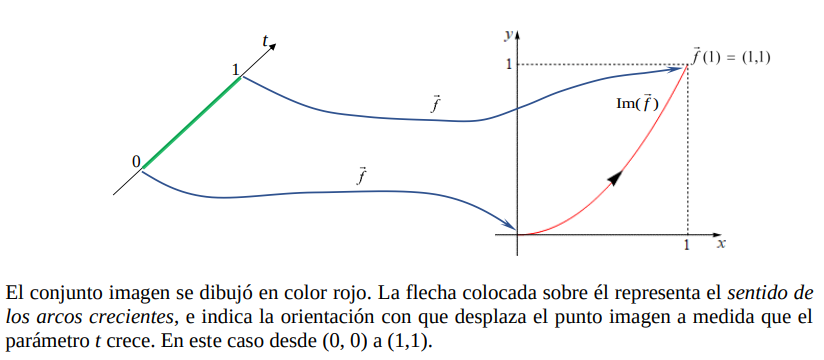
\includegraphics[width=0.8\textwidth]{img/2.3ej.png}
    \caption{Dada $\vec{f}:[0,1] \in R \to R^2 / \vec{f}(t) = (t, t^2)$, represente el correspondiente conjunto imagen.}
    \label{fig:2.3ej}
\end{figure}